\documentclass{standalone}
\usepackage{tikz}
\usetikzlibrary{patterns, positioning}


\begin{document}
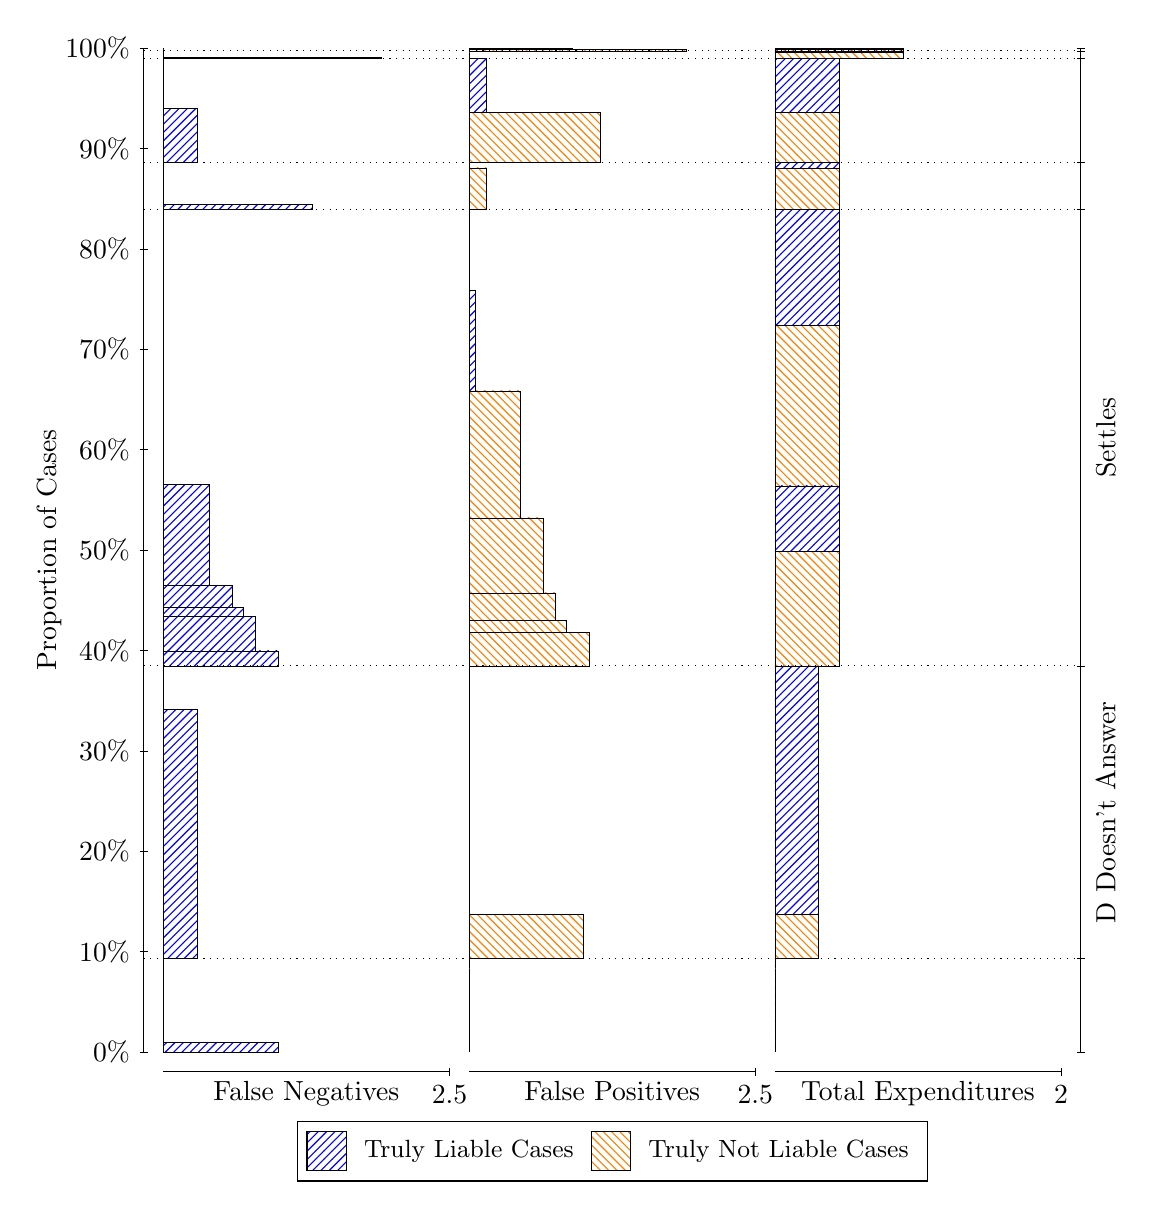
\begin{tikzpicture}
\draw[black, very thin] (1.5,1.75) -- (1.5,14.5);
\node[rotate=90, text=black, anchor=center] at (0.3, 8.125) {Proportion of Cases};
\draw[black, very thin] (1.45,1.75) -- (1.55,1.75);
\node[text=black, anchor=east] at (1.45, 1.75) {0\%};
\draw[black, very thin] (1.45,3.025) -- (1.55,3.025);
\node[text=black, anchor=east] at (1.45, 3.025) {10\%};
\draw[black, very thin] (1.45,4.3) -- (1.55,4.3);
\node[text=black, anchor=east] at (1.45, 4.3) {20\%};
\draw[black, very thin] (1.45,5.575) -- (1.55,5.575);
\node[text=black, anchor=east] at (1.45, 5.575) {30\%};
\draw[black, very thin] (1.45,6.85) -- (1.55,6.85);
\node[text=black, anchor=east] at (1.45, 6.85) {40\%};
\draw[black, very thin] (1.45,8.125) -- (1.55,8.125);
\node[text=black, anchor=east] at (1.45, 8.125) {50\%};
\draw[black, very thin] (1.45,9.4) -- (1.55,9.4);
\node[text=black, anchor=east] at (1.45, 9.4) {60\%};
\draw[black, very thin] (1.45,10.675) -- (1.55,10.675);
\node[text=black, anchor=east] at (1.45, 10.675) {70\%};
\draw[black, very thin] (1.45,11.95) -- (1.55,11.95);
\node[text=black, anchor=east] at (1.45, 11.95) {80\%};
\draw[black, very thin] (1.45,13.225) -- (1.55,13.225);
\node[text=black, anchor=east] at (1.45, 13.225) {90\%};
\draw[black, very thin] (1.45,14.5) -- (1.55,14.5);
\node[text=black, anchor=east] at (1.45, 14.5) {100\%};

\draw[black, very thin] (13.4,1.75) -- (13.4,14.5);
\draw[black, very thin] (13.35,1.75) -- (13.45,1.75);
\node[anchor=west] at (13.35, 1.75) {};
\draw[black, very thin] (13.35,2.9362) -- (13.45,2.9362);
\node[anchor=west] at (13.35, 2.9362) {};
\draw[black, very thin] (13.35,6.6538) -- (13.45,6.6538);
\node[anchor=west] at (13.35, 6.6538) {};
\draw[black, very thin] (13.35,12.446) -- (13.45,12.446);
\node[anchor=west] at (13.35, 12.446) {};
\draw[black, very thin] (13.35,13.049) -- (13.45,13.049);
\node[anchor=west] at (13.35, 13.049) {};
\draw[black, very thin] (13.35,14.364) -- (13.45,14.364);
\node[anchor=west] at (13.35, 14.364) {};
\draw[black, very thin] (13.35,14.465) -- (13.45,14.465);
\node[anchor=west] at (13.35, 14.465) {};
\draw[black, very thin] (13.35,14.5) -- (13.45,14.5);
\node[anchor=west] at (13.35, 14.5) {};

\draw[black, very thin, pattern color=blue, pattern=north east lines] (1.75,1.75) rectangle (3.2033,1.8748);
\draw[black, very thin, pattern color=orange, pattern=north west lines] (1.75,1.8748) rectangle (1.75,2.9362);
\draw[black, very thin, pattern color=blue, pattern=north east lines] (1.75,2.9362) rectangle (2.186,6.0961);
\draw[black, very thin, pattern color=orange, pattern=north west lines] (1.75,6.0961) rectangle (1.75,6.6538);
\draw[black, very thin, pattern color=blue, pattern=north east lines] (1.75,6.6538) rectangle (3.2033,6.8451);
\draw[black, very thin, pattern color=blue, pattern=north east lines] (1.75,6.8451) rectangle (2.9127,7.2802);
\draw[black, very thin, pattern color=blue, pattern=north east lines] (1.75,7.2802) rectangle (2.7673,7.401);
\draw[black, very thin, pattern color=blue, pattern=north east lines] (1.75,7.401) rectangle (2.622,7.6733);
\draw[black, very thin, pattern color=blue, pattern=north east lines] (1.75,7.6733) rectangle (2.3313,8.9545);
\draw[black, very thin, pattern color=orange, pattern=north west lines] (1.75,8.9545) rectangle (1.75,12.446);
\draw[black, very thin, pattern color=blue, pattern=north east lines] (1.75,12.446) rectangle (3.6393,12.518);
\draw[black, very thin, pattern color=orange, pattern=north west lines] (1.75,12.518) rectangle (1.75,13.049);
\draw[black, very thin, pattern color=blue, pattern=north east lines] (1.75,13.049) rectangle (2.186,13.731);
\draw[black, very thin, pattern color=orange, pattern=north west lines] (1.75,13.731) rectangle (1.75,14.364);
\draw[black, very thin, pattern color=blue, pattern=north east lines] (1.75,14.364) rectangle (4.5113,14.384);
\draw[black, very thin, pattern color=orange, pattern=north west lines] (1.75,14.384) rectangle (1.75,14.465);
\draw[black, very thin, pattern color=orange, pattern=north west lines] (1.75,14.465) rectangle (1.75,14.484);
\draw[black, very thin, pattern color=blue, pattern=north east lines] (1.75,14.484) rectangle (1.75,14.5);
\draw[black, very thin, pattern color=orange, pattern=north west lines] (5.6333,1.75) rectangle (5.6333,2.8114);
\draw[black, very thin, pattern color=blue, pattern=north east lines] (5.6333,2.8114) rectangle (5.6333,2.9362);
\draw[black, very thin, pattern color=orange, pattern=north west lines] (5.6333,2.9362) rectangle (7.0867,3.4939);
\draw[black, very thin, pattern color=blue, pattern=north east lines] (5.6333,3.4939) rectangle (5.6333,6.6538);
\draw[black, very thin, pattern color=orange, pattern=north west lines] (5.6333,6.6538) rectangle (7.1593,7.0746);
\draw[black, very thin, pattern color=orange, pattern=north west lines] (5.6333,7.0746) rectangle (6.8687,7.2354);
\draw[black, very thin, pattern color=orange, pattern=north west lines] (5.6333,7.2354) rectangle (6.7233,7.5815);
\draw[black, very thin, pattern color=orange, pattern=north west lines] (5.6333,7.5815) rectangle (6.578,8.5331);
\draw[black, very thin, pattern color=orange, pattern=north west lines] (5.6333,8.5331) rectangle (6.2873,10.145);
\draw[black, very thin, pattern color=blue, pattern=north east lines] (5.6333,10.145) rectangle (5.706,11.426);
\draw[black, very thin, pattern color=blue, pattern=north east lines] (5.6333,11.426) rectangle (5.6333,12.446);
\draw[black, very thin, pattern color=orange, pattern=north west lines] (5.6333,12.446) rectangle (5.8513,12.977);
\draw[black, very thin, pattern color=blue, pattern=north east lines] (5.6333,12.977) rectangle (5.6333,13.049);
\draw[black, very thin, pattern color=orange, pattern=north west lines] (5.6333,13.049) rectangle (7.3047,13.683);
\draw[black, very thin, pattern color=blue, pattern=north east lines] (5.6333,13.683) rectangle (5.8513,14.364);
\draw[black, very thin, pattern color=orange, pattern=north west lines] (5.6333,14.364) rectangle (5.6333,14.445);
\draw[black, very thin, pattern color=blue, pattern=north east lines] (5.6333,14.445) rectangle (5.6333,14.465);
\draw[black, very thin, pattern color=orange, pattern=north west lines] (5.6333,14.465) rectangle (8.3947,14.484);
\draw[black, very thin, pattern color=blue, pattern=north east lines] (5.6333,14.484) rectangle (6.9413,14.5);
\draw[black, very thin, pattern color=orange, pattern=north west lines] (9.5167,1.75) rectangle (9.5167,2.8114);
\draw[black, very thin, pattern color=blue, pattern=north east lines] (9.5167,2.8114) rectangle (9.5167,2.9362);
\draw[black, very thin, pattern color=orange, pattern=north west lines] (9.5167,2.9362) rectangle (10.062,3.4939);
\draw[black, very thin, pattern color=blue, pattern=north east lines] (9.5167,3.4939) rectangle (10.062,6.6538);
\draw[black, very thin, pattern color=orange, pattern=north west lines] (9.5167,6.6538) rectangle (10.334,8.1123);
\draw[black, very thin, pattern color=blue, pattern=north east lines] (9.5167,8.1123) rectangle (10.334,8.9405);
\draw[black, very thin, pattern color=orange, pattern=north west lines] (9.5167,8.9405) rectangle (10.334,10.973);
\draw[black, very thin, pattern color=blue, pattern=north east lines] (9.5167,10.973) rectangle (10.334,12.446);
\draw[black, very thin, pattern color=orange, pattern=north west lines] (9.5167,12.446) rectangle (10.334,12.977);
\draw[black, very thin, pattern color=blue, pattern=north east lines] (9.5167,12.977) rectangle (10.334,13.049);
\draw[black, very thin, pattern color=orange, pattern=north west lines] (9.5167,13.049) rectangle (10.334,13.683);
\draw[black, very thin, pattern color=blue, pattern=north east lines] (9.5167,13.683) rectangle (10.334,14.364);
\draw[black, very thin, pattern color=orange, pattern=north west lines] (9.5167,14.364) rectangle (11.152,14.445);
\draw[black, very thin, pattern color=blue, pattern=north east lines] (9.5167,14.445) rectangle (11.152,14.465);
\draw[black, very thin, pattern color=orange, pattern=north west lines] (9.5167,14.465) rectangle (11.152,14.484);
\draw[black, very thin, pattern color=blue, pattern=north east lines] (9.5167,14.484) rectangle (11.152,14.5);
\draw[black, dotted] (1.5,2.9362) -- (13.4,2.9362);
\draw[black, dotted] (1.5,6.6538) -- (13.4,6.6538);
\draw[black, dotted] (1.5,12.446) -- (13.4,12.446);
\draw[black, dotted] (1.5,13.049) -- (13.4,13.049);
\draw[black, dotted] (1.5,14.364) -- (13.4,14.364);
\draw[black, dotted] (1.5,14.465) -- (13.4,14.465);
\draw[black, very thin] (1.75,1.5) -- (5.3833,1.5);
\node[text=black, anchor=north] at (3.5667, 1.5) {False Negatives};
\draw[black, very thin] (5.3833,1.45) -- (5.3833,1.55);
\node[text=black, anchor=north] at (5.3833, 1.45) {2.5};

\draw[black, very thin] (5.6333,1.5) -- (9.2667,1.5);
\node[text=black, anchor=north] at (7.45, 1.5) {False Positives};
\draw[black, very thin] (9.2667,1.45) -- (9.2667,1.55);
\node[text=black, anchor=north] at (9.2667, 1.45) {2.5};

\draw[black, very thin] (9.5167,1.5) -- (13.15,1.5);
\node[text=black, anchor=north] at (11.333, 1.5) {Total Expenditures};
\draw[black, very thin] (13.15,1.45) -- (13.15,1.55);
\node[text=black, anchor=north] at (13.15, 1.45) {2};


\node[text=black, centered, rotate=90] at (13.72, 4.795) {D Doesn't Answer};
\node[text=black, centered, rotate=90] at (13.72, 9.5498) {Settles};





\draw (7.449999999999999,1.5) node[draw=none] (baseCoordinate) {};
\begin{scope}[align=center]
        \matrix[scale=0.5, draw=black, below=0.5cm of baseCoordinate, nodes={draw}, column sep=0.1cm]{
            \node[rectangle, draw, minimum width=0.5cm, minimum height=0.5cm, pattern color=blue, pattern=north east lines] {}; &
            \node[draw=none, font=\small, text=black] (B) {Truly Liable Cases}; &
            \node[rectangle, draw, minimum width=0.5cm, minimum height=0.5cm, pattern color=orange, pattern=north west lines] {}; &
            \node[draw=none, font=\small, text=black] (B) {Truly Not Liable Cases}; \\
            };
\end{scope}

\end{tikzpicture}
\end{document}